    \section{Tesla Motors}

\subsection{A little bit of history}
\begin{frame}
\frametitle{A little bit of history}
\begin{itemize}
    \itemsep1em
    \item Cars were powered by electricity in 1903
        % Invented the electric starter to just keep the noise inconvenience
        % compared to electrical motors
    \item Ford needed to reduce its car production cost
    \item Inventing a new way to produce faster % mass production
    \item Seems to have worked since 1908 and the Ford T
    \item No product advertisement was needed between 1917 and 1923
\end{itemize}
\end{frame}

\subsection{One weird kid in the playground}
\begin{frame}
\frametitle{Everyone sees the potential of electric cars}
\begin{itemize}
    \itemsep1.5em
    \item Smooth feeling on the road
    \item Decreasing oil dependency
    \item Reduces the pollution released compares to classic cars
    \item Everybody seems to agree that it is the future car
\end{itemize}
\end{frame}

\begin{frame}
\frametitle{But…}
\begin{itemize}
    \itemsep1.5em
    \item What about the autonomy?
    \item Driving might be slow… no?
    \item Reducing the pollution… really? % preconceived ideas
    \item Does it have to be today? Not… like… in 20 years?
\end{itemize}
\end{frame}

\begin{frame}
\frametitle{No one wants electric cars to be on market}
\begin{itemize}
    \itemsep1.5em
    \item Selling gasoline-based cars would be difficult % 10 parts compared to 200
    \item Requiring more investments
    \item Lobbying by the oil industry  % case with the BBC
    \item Governments are not pushing it enough % because they impose taxes on
        % oil and do not want to afraid "classic" constructors. Plus, the US is
        % a big oil producer
\end{itemize}
\end{frame}


\subsection{Autonomy is a real issue}

\begin{frame}
\frametitle{The autonomy is the real issue}
\begin{itemize}
    \itemsep1.5em
    \item AC Propulsion
    \item Maximum range: 250 miles
    \item No station to charge the car
    \item The most criticized point
\end{itemize}
\end{frame}

\begin{frame}
\frametitle{Superchargers}
\begin{itemize}
    \itemsep1.5em
    \item 60 miles of range for every 10 minutes
    \item Battery swap, \$60--\$80
    \item Fast or free
    \item US\@: 1,346 stations, 224 supercharger locations
    \item 500 Supercharger locations
\end{itemize}
\end{frame}


\begin{frame}
\frametitle{Solarcity and batteries factory}
\begin{itemize}
    \itemsep1.5em
    \item Tesla Gigafactory 1 % In the nevada
    \item Slated to be operational in 2017
    \item Reduce batteries production cost by at least 30\%
    \item More than 30GWh/year
\end{itemize}
\end{frame}


\begin{frame}
\begin{center}
\begin{columns}
\begin{column}{330px}
{
    \begin{figure}[h!]
        \centering
        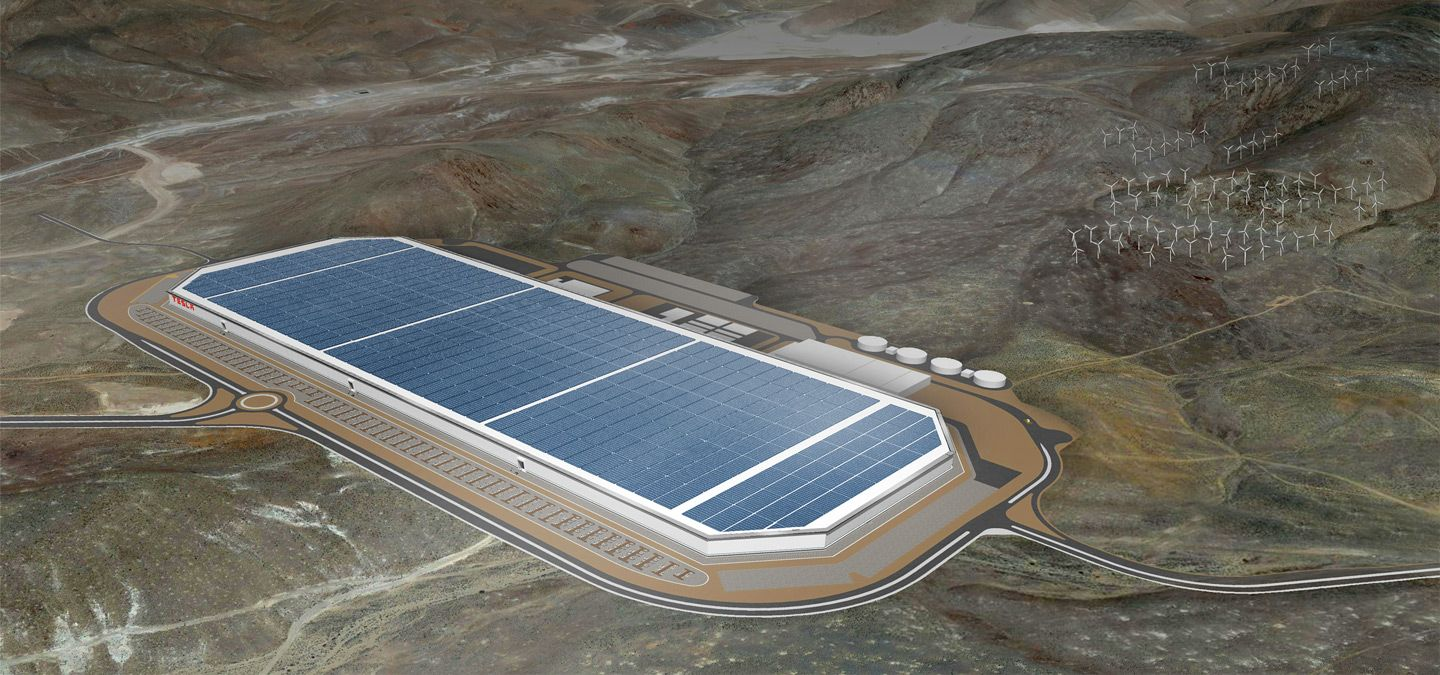
\includegraphics[width=310px]
            {images/tesla-gigafactory.jpg}
        \caption{Tesla Gigafactory1}
        \scriptsize{Source :
            \url{http://www.teslamotors.com}}
    \end{figure}
}
\end{column}
\end{columns}
\end{center}
\end{frame}


\begin{frame}
\frametitle{Hyperloop}
\begin{itemize}
    \itemsep2em
    \begin{columns}
        \begin{column}{39mm}
            \item Between train and planes
            \item 800miles/h (1200km/h)
        \end{column}
        \begin{column}{36mm}
            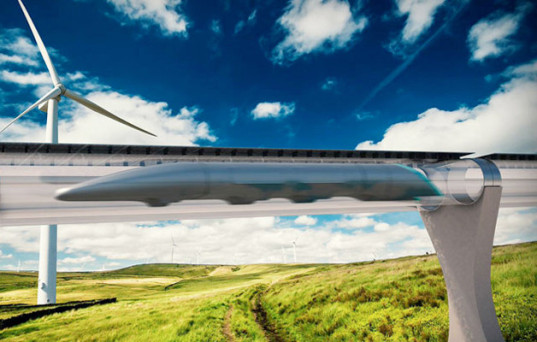
\includegraphics[width=48mm]{images/hyperloop.jpg}
        \end{column}
    \end{columns}
    \item Los Angeles -- San Francisco in 35mn (354 miles -- 570km)
\end{itemize}
\end{frame}


\subsection{A plan in 3 big steps}

{
\logo{}
\begin{frame}
\frametitle{Electric cars can be cool}
\begin{center}
\begin{columns}
\begin{column}{330px}
{
    \begin{figure}[h!]
        \centering
        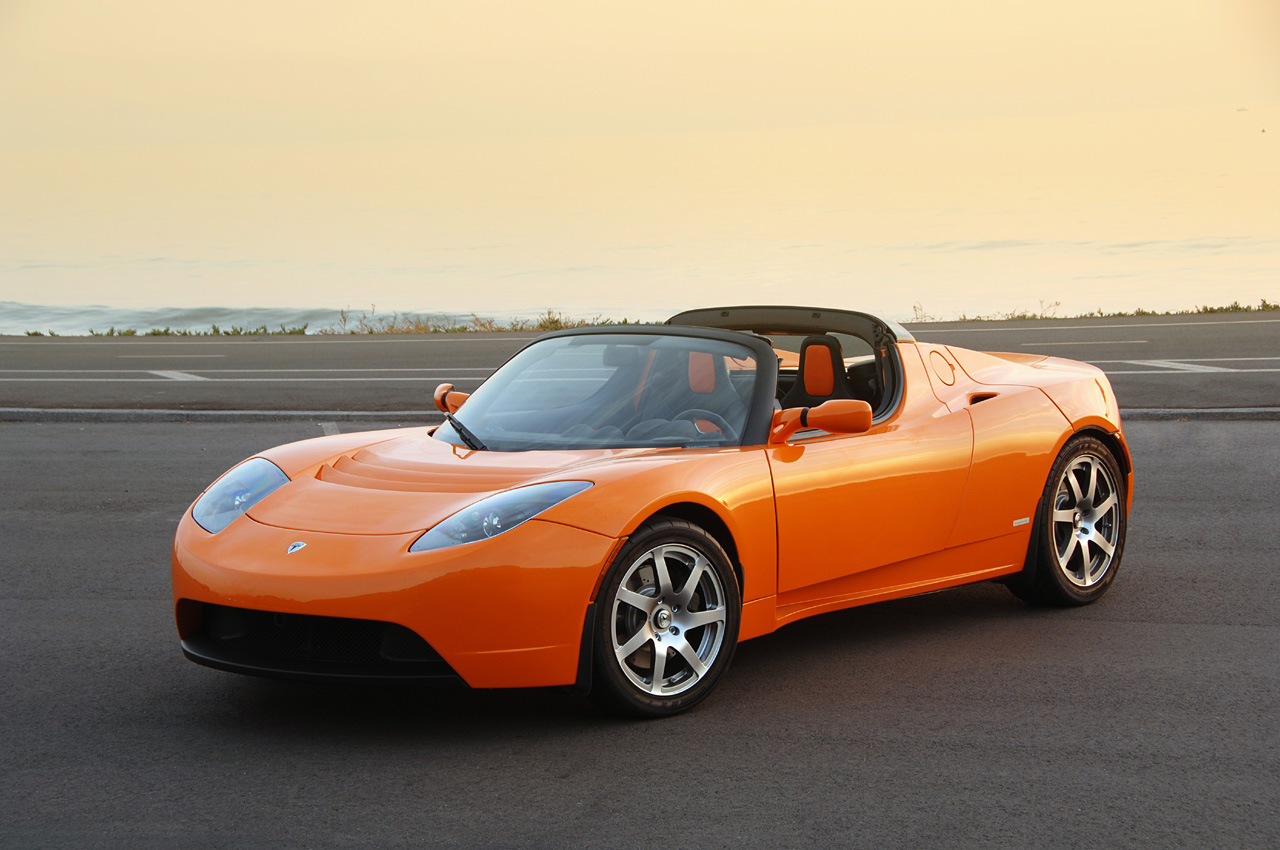
\includegraphics[width=250px]
            {images/tesla-roadster.jpg}
        \caption{Tesla Roadster}
    \end{figure}
}
\end{column}
\end{columns}
\end{center}
\end{frame}
}

\begin{frame}
\begin{itemize}
    \itemsep1.5em
    \item Tesla Roadster Sport
    \item Powerful: 0--60 mph in 3.70 seconds
    \item Range: 244 miles (393km)
    \item No compromise
    \item US \$128,500
    % At this step, Musk has to reinvest a big part of his money or tesla would
    % die
\end{itemize}
\end{frame}

\begin{frame}
\begin{itemize}
    \itemsep1.5em
    \item Efficiency of battery-to-wheel motor: 88\% on average
        % For comparison, internal combustion engines have a tank-to-wheel
        % efficiency of about 15%
        % https://en.wikipedia.org/wiki/Tesla_Roadster#Energy_efficiency
    \item Regular cool free upgrades
    \item 1\textsuperscript{st} automobile constructor in Silicon Valley
    \item Loads of gadgets
\end{itemize}
\end{frame}

{
\logo{}
\begin{frame}
\frametitle{Electric cars can be classy}
\begin{center}
\begin{columns}
\begin{column}{330px}
{
    \begin{figure}[h!]
        \centering
        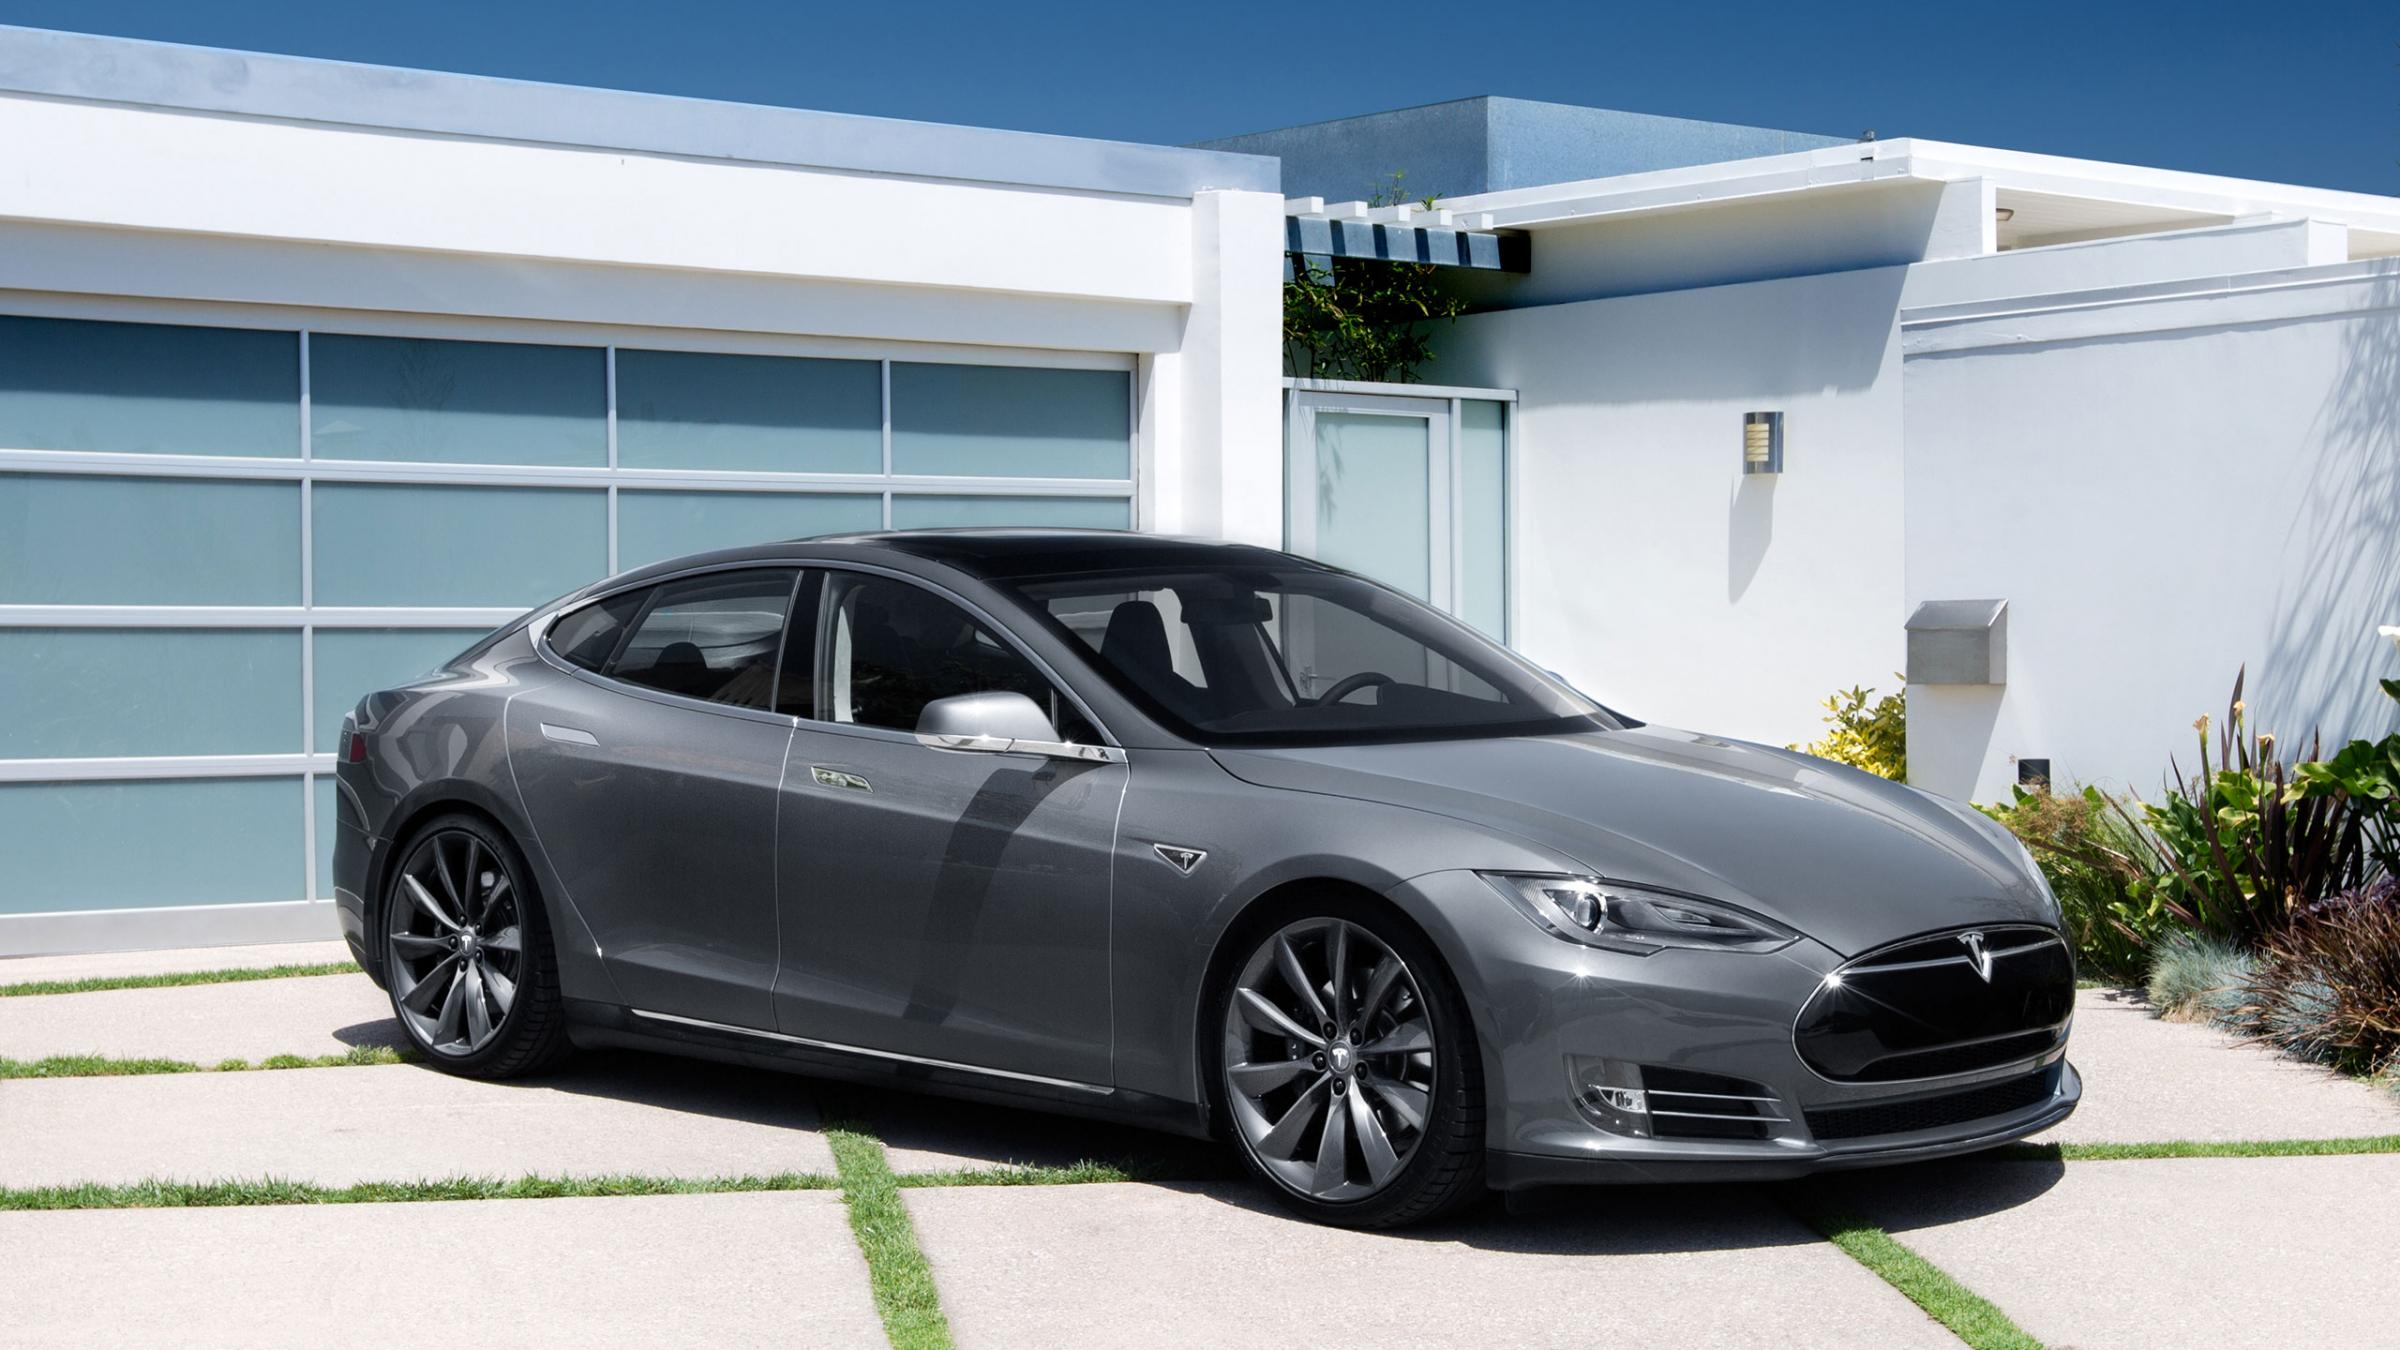
\includegraphics[width=300px]
            {images/tesla-model-s.jpg}
        \vspace{-0.5em}
        \caption{Tesla Model S}
    \end{figure}
}
\end{column}
\end{columns}
\end{center}
\end{frame}
}


{
\logo{}
\begin{frame}
\begin{center}
\begin{columns}
\begin{column}{330px}
{
    \begin{figure}[h!]
        \centering
        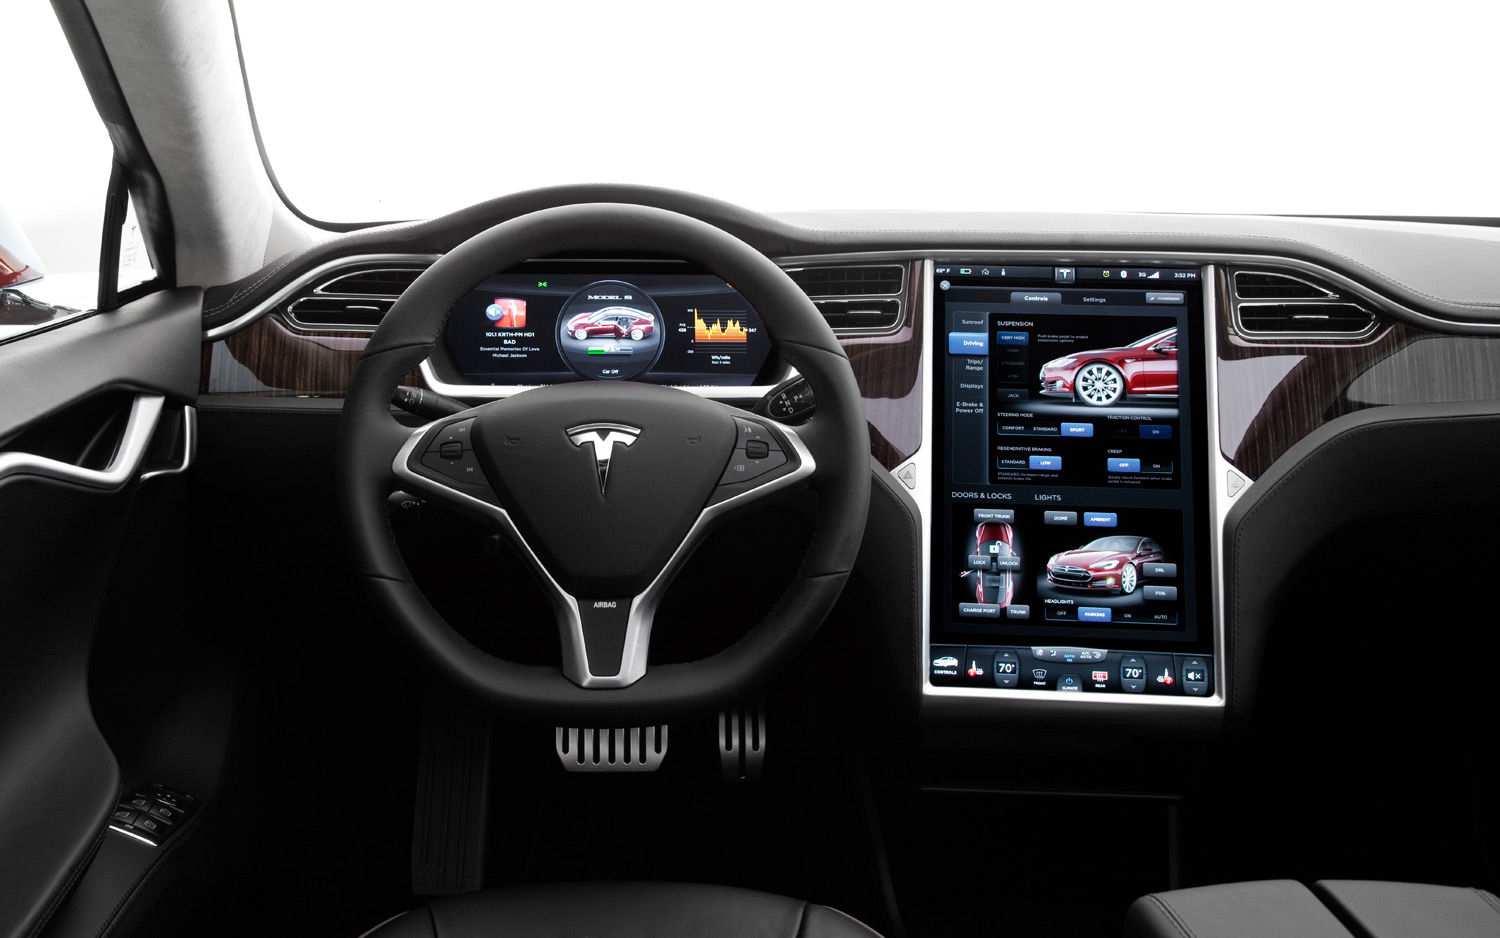
\includegraphics[width=300px]
            {images/tesla-model-s-cockpit.jpg}
        \vspace{-0.5em}
        \caption{Tesla Model S cockpit}
    \end{figure}
}
\end{column}
\end{columns}
\end{center}
\end{frame}
}


\begin{frame}
\begin{itemize}
    \itemsep1.5em
    \item Model S and then Model X
    \item More ``affordable'': US\$80,000
    \item Range: 320 miles (520km)
    \item Autopilot and cool features
\end{itemize}
\end{frame}

\begin{frame}
\frametitle{Electric cars for the mass}
\begin{itemize}
    \itemsep1.5em
    \item Model 3
    \item Scheduled for 2017
    \item Expected cost: around US\$35,000
    \item Government's \$7500 EV tax credit
\end{itemize}
\end{frame}
